%% SECTION HEADER /////////////////////////////////////////////////////////////////////////////////////
\section{Sandwich composite structure}
\label{sec:scs}

%% SECTION CONTENT ////////////////////////////////////////////////////////////////////////////////////
Composites consist of two or more different materials, such as plastics, resins, metal alloys, glass, carbon or bio-based fibres. The combination of material constituents gives  structure benefits from the properties of the component materials, e.g., the strength of carbon fibres and the low density of the polymer resin in the case of \ac{cfrp}.
The contribution of lightweight composite materials to the production of structural components has been increasing rapidly since the middle of the last century.
Due to the high strength-to-weight ratio, higher operating temperatures, greater stiffness and higher
reliability, composite materials are extensively used in the aircraft and aerospace industry and civil constructions.
Composites account for more than 50\% of the total weight of the aircraft Boeing 787 and Airbus A350 \cite{giurgiutiu2015structural}.

One group of composites includes sandwich panels, which is a type of multi-layered structure that are composed of the mid-core sandwiched between thin skins.
The skins, made of high strength materials, are designed to carry tensile or compressive stresses from longitudinal forces and bending moments.
On the other hand, the core transmits mainly shear stresses from transverse forces.
It also separates the skins, which increases structural stiffness for thin layers, improves insulation properties, and reduces weight while maintaining strength properties similar to the solid construction of the same density.
A popular core used in engineering structures is a honeycomb geometry core.
Fig.~\ref{fig:hcp} shows the construction of the \ac{hsc}.
The core can be made of aluminium, cardboard or Nomex. 
\begin{figure}[H] %hbtp
	\begin{center}
		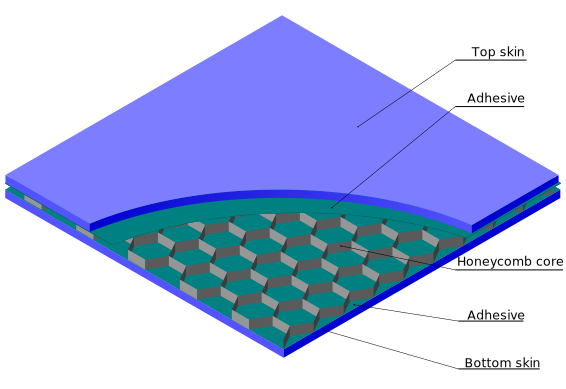
\includegraphics[width=0.95\textwidth]{Intro/honeycomb_plate}
		\caption{
			\label{fig:hcp} Structure of the honeycomb sandwich composite.}
		\vspace{-0.5cm}
	\end{center}
\end{figure}

However, these complex structures are exposed to various types of damage that are not found in metal alloy materials, e.g., hidden disbonds between the skin and the core, delamination of the composite skins, or the core impact damage.
They can occur either during a manufacturing process, storage or in-service life.
Therefore, advanced methods are required for online damage detection.
Thus, the use of composites has motivated the development of advanced approaches to structural inspections, e.g., methods based on elastic wave propagation had to account for the anisotropic structure of the material.